\documentclass[../paper.tex]{subfiles}
\begin{document}
M-Theory is a theory based on the concept that spacetime has 10 dimensions. This concept only works under the postulate that 6 of these 10 dimension for a compact manifold, M. Within M-Theory, the observable universe (so the universe as we know and observe it) exists within a higher-dimensional (in this case 6 dimensional) manifold. An example for one of these manifolds is the Calabi Yau Manifold, as shown in figure \ref{Calabi Yau}. 

\begin{figure}[!htb]
\centering
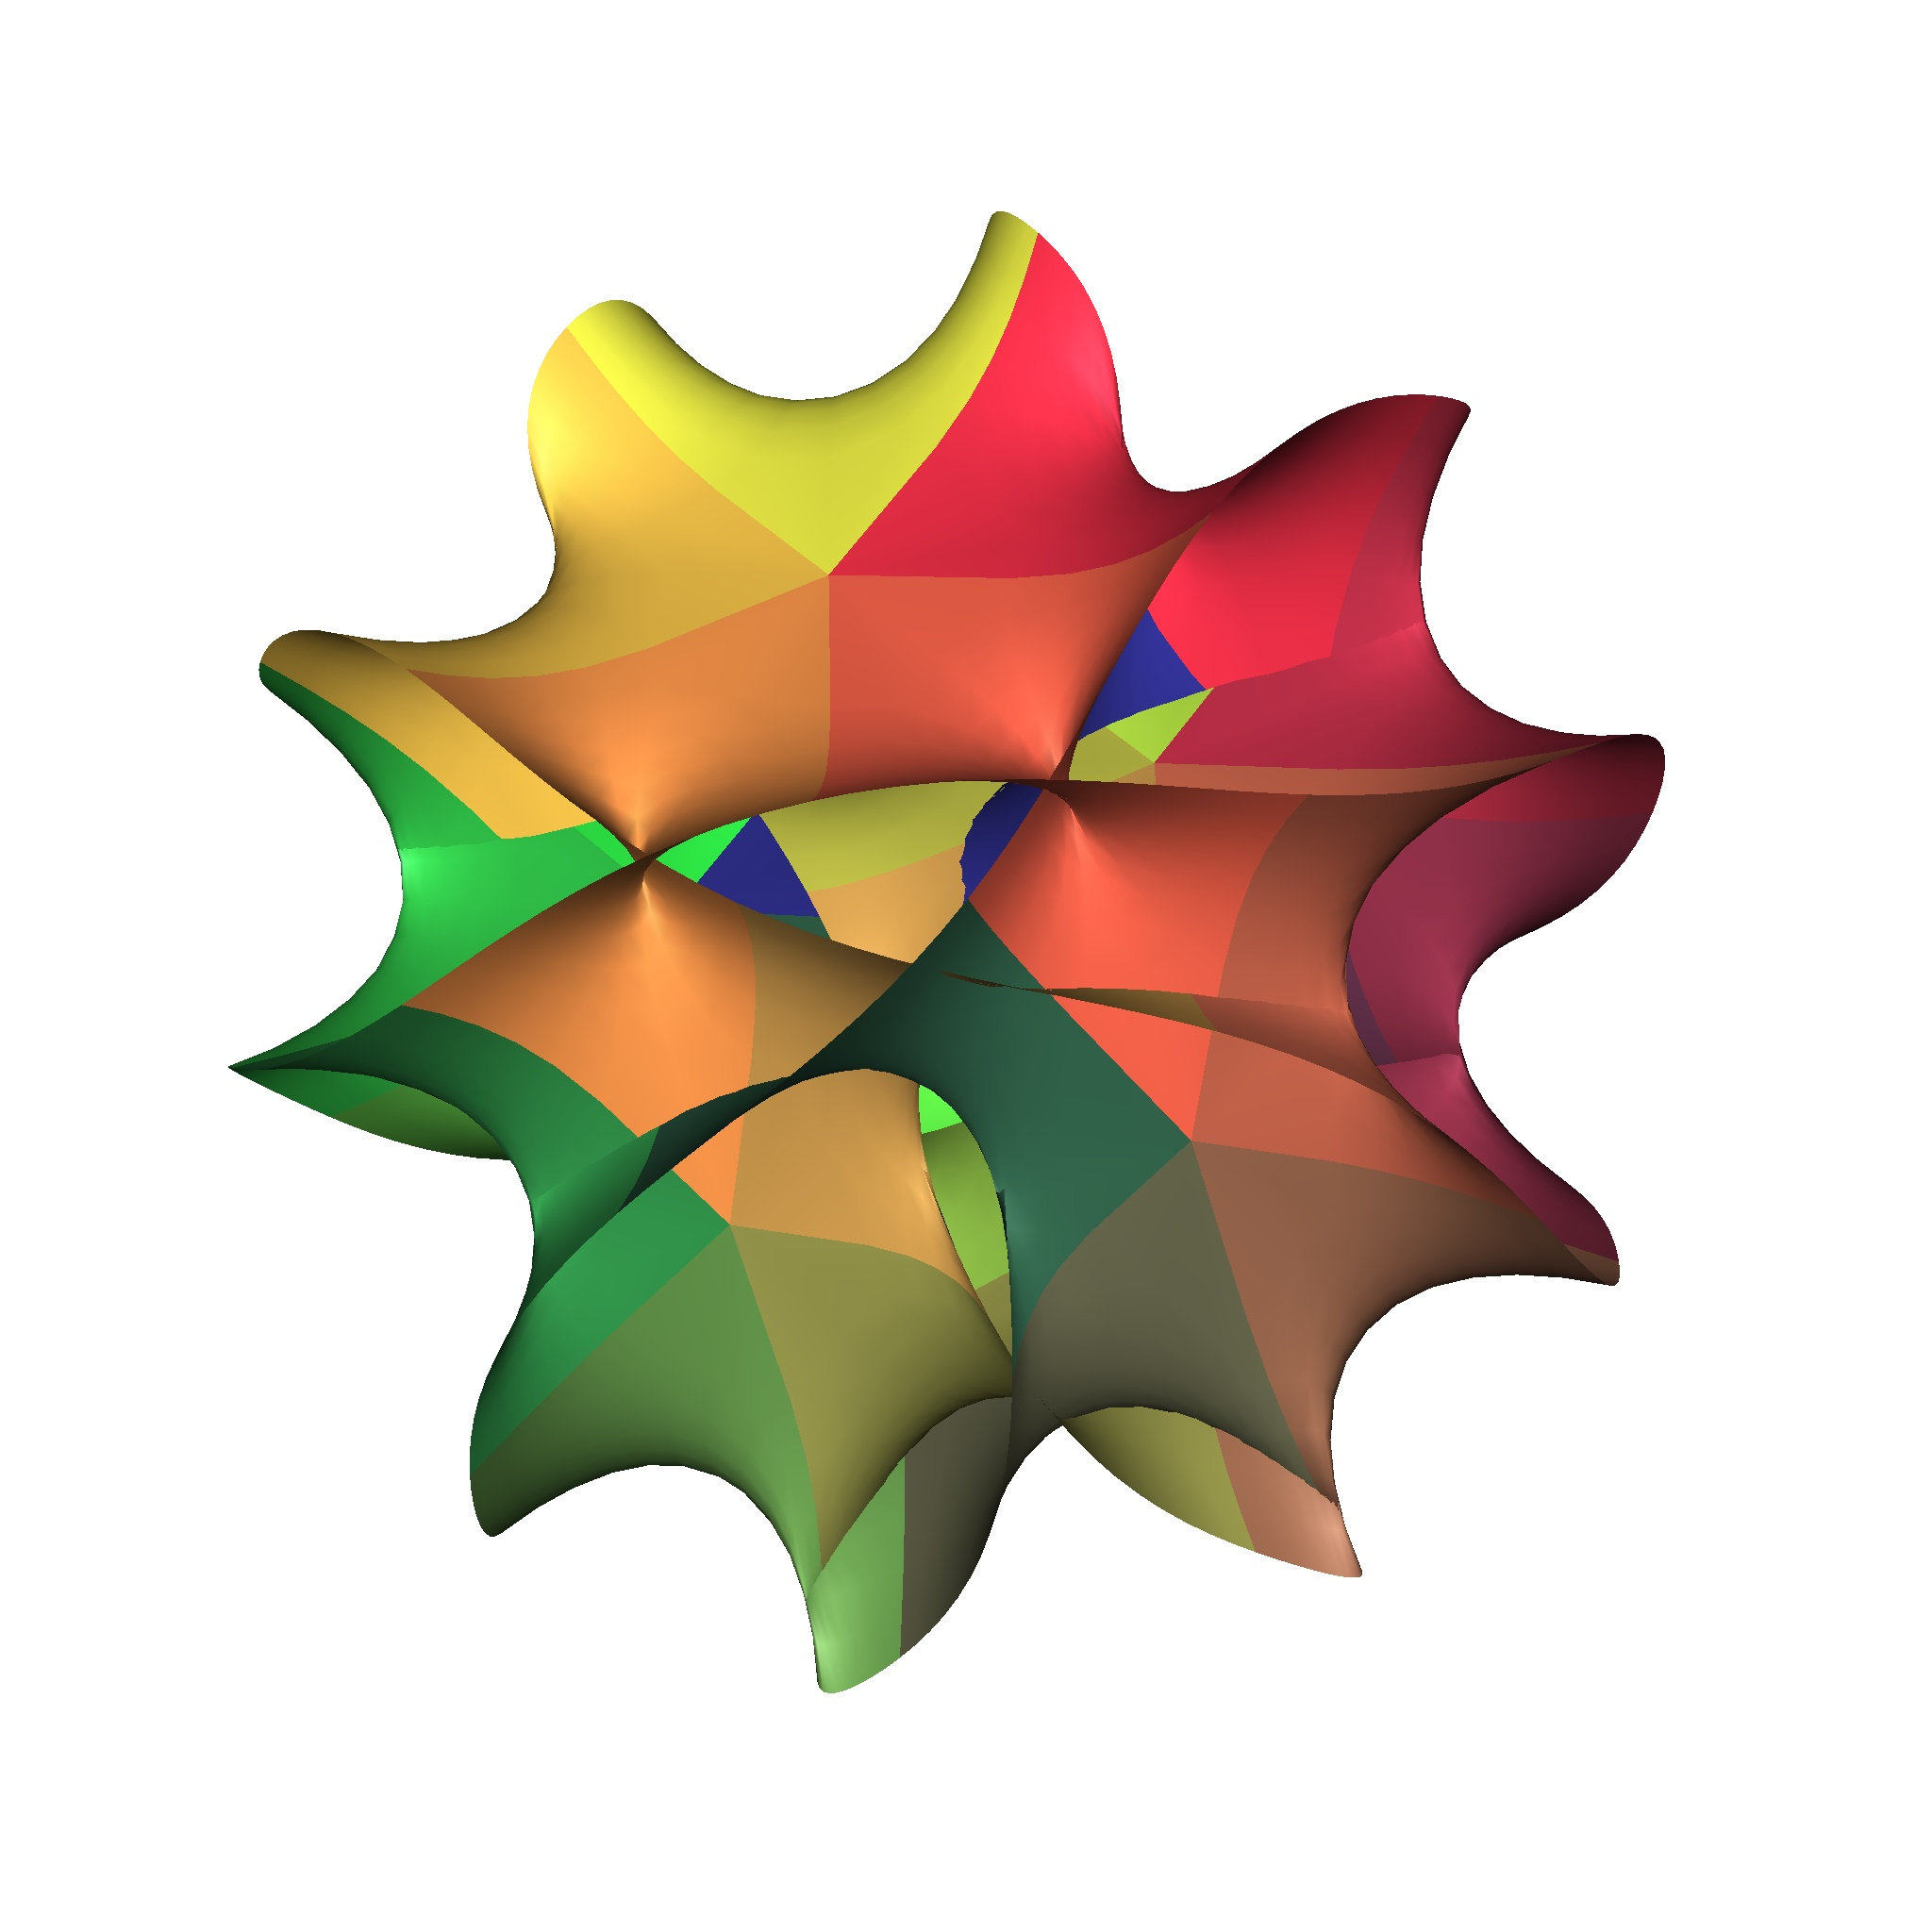
\includegraphics[scale = 0.1]{M-Theory/calabiyau.jpg}
\caption{Calabi Yau Manifold}
\label{Calabi Yau}
\end{figure}

This is not contradicting current experience, but only under the postulate that M has a diameter much less than a micron. There are many shapes for M which can be chosen. For each shape M, 4 additional dimensions can be chosen. These 4, for example branch, flux and others,  will be called V. Since the a priori probability for each of these shape predicting objects isn't known, for each shape a theory can be derived for predicting the physics in the universe. After defining M and V, the theory of strings vibrating on M needs to be worked out. Certain properties such as the matter and forces of the object M can be obtained by it's topology and geometry. The strings vibrating on the object should give the properties of the object, if String Theory is true and the correct values for M and V are being chosen. If the predictions correspond with the actual values, the probability of the current model will increase. There is strong evidence that the combinations for M and V are finite. If there really is a finite amount of combinations, String Theory can be falsified by computational exploration. In order for this to happen, every single combination has to be proven false by predicting the universe as we currently know it. Even though String Theory may be falsified by computational exploration,, proving String Theory this way is a lot harder, if even possible. String Theory must describe every single aspect in the whole universe. Let's say there's a finite number of Laws of Nature. String Theory has to be proving all the Laws of Nature. As long as mankind doesn't know if they found all Laws of Nature, we cannot justify a computational proof of String Theory, since we simply don't know if it applies to all Laws of Nature. If there would be a infinite amount of Laws of Nature (which sounds like a paradox), it would be completely impossible to proof the theory by using computational exploration. Considering these possibilities, for every possible combination (M,V) it would be ideal if a probability distribution can be derived as in Equation \ref{Probability}.

\begin{equation}
    P(m,v)
    \label{Probability}
\end{equation}

In order to obtain this probability distribution a lot, and preferably all, of the combinations for (M,V) should be looked into. This is a computational problem, since the structures M and V are very complex and there are a lot of unique values. The computational side of the problem will be discussed later on.

\end{document}